\section{Motivation and Problem Statement}

Internet of Things (IoT)~\index{IoT}, also known as Internet of Everything (IoE)~\index{IoE}, is a novel paradigm that rapidly gains vast attention in the internet era. The basic idea of IoT is the inter-networking of variety of ``Things''~\index{IoT Things} through unique addressing scheme, while ``Things'' is an precisely identifiable object - such sensors, actuators, connected tags, mobile phones, etc.~\cite{atzori2010internet}\cite{bassi2008internet}. 
The Internet of Things aims to create a smart environment by bringing the Things from physical world into digital world. In other word, IoT is not only connecting to the Things using the Internet but also enabling data exchange. Ideally, everything could be connected anytime from anywhere by anyone. Based on such context, the massive number of innovative applications has been emerging to exploit the benefits of connectivity and accessibility of everything~\cite{vermesan2013internet}. For example, there will be intelligent cities, transform business process from production line to retail delivery by providing real-time monitoring flow of products~\cite{lee2015internet}.\\

It is not surprising that IoT is considered as a new revolution of the internet that highly affects several real-life aspects. From an individual user view, the internet of things enhances the life quality by offering smart transportation, e-health or smart home. Similarly, from a business view, the IoT opens ideal opportunities in industrial fields such as automation and manufacturing, logistic \cite{2010}. US National Intelligence Council listed IoT as one of the six ``Disruptive Civil technology'' potentially impacted US national power \cite{intelligence2008six}. The number of Internet-connected devices exceeded the number of human beings on the planet in 2011, by the end of 2020, 212 billion IoT smart objects will be deployed worldwide and by 2025, everyday things will be connected to Internet such as food containers, furniture, paper documents, and more \cite{floyer2013defining}\cite{TheInter38:online}.\\

Despite producing infinite opportunities in every-day life aspects, IoT is still facing many critical challenges relating data interoperation, interpretation and the formation of knowledge. This is powered by the fact that the raw data collected from IoT Things is massive, heterogeneous and contains vast amount of redundant information. Dealing with these challenges, the IoT service providers have been seeking innovative solutions to effectively collect, process, analyze and present meaningfully IoT data. On the other hand, cloud computing is emerging as a disruptive technology which unlimitedly provides storage and processing power capabilities. Taking these advantages may partially solve most of the IoT issues. Thus, the integration between IoT and cloud computing creates a novel IT paradigm named CloudIoT or cloud-based IoT~\cite{fox2012architecture}\cite{dash2010survey}\cite{suciu2013smart}. 

In general, IoT can leverage the unlimited storage capabilities and processing of Cloud to bridge its technological gaps (e.g. constrained storage, processing power, and communication). For example, Cloud can provide the effective solutions to storage the IoT data that is more secure and easily accesses from anywhere. In many cases, cloud acts as intermediate layer between the Things and applications to hide the complexity and heterogeneity of Thing's technologies. This will facilitate the IoT application development and deployment. However, information gathering, processing and transmission through cloud will arise many challenges~\cite{aguzzi2013definition}. Two of those challenges targeted in our works are heterogeneity and reliability.   \\

\par \textbf{Interoperability: } The most critical challenge in CloudIoT is lack of unique standard in several elements from devices, platforms, services to applications~\cite{bandyopadhyay2011internet}. In addition, CloudIoT platforms have been typically designed as isolated vertical solutions for specific purposes~\cite{dinh2013survey}. To integrate with these platforms, the IoT providers must analyze in detail requirements about hardware, software, subsystems that tightly specialized in the application context. On the other hand, new IoT device types along with their own data format are emerging every day. This leads to a big challenge of heterogeneity while deploying IoT solutions in large-scale. Even though the scientific community has provided multiple contributions relating standardization, it is clearly necessary of unified architecture, mechanisms, standard Things descriptions to facilitate the connection to heterogeneous Things, transform and present collected data under usable knowledge~\cite{Botta2016}.\\

\par\textbf{Reliability: } Many of IoT applications are business critical, and strongly require the underlying technology to be reliable. That means these application must deliver high-quality services even in the presence of the failures in collected data. In additions, energy consumption of IoT devices also highly impacts in the overall system reliability. 

\begin{itemize}

    \item \textbf{Data reliability: }As consequences of rapid growth, there is a vast amount of raw data being continuously collected from billions of interconnected devices. The flow of such data will widen human awareness about the natural phenomenon, living environment or entity through intelligent services.  However, IoT data are generally unreliable due to strongly affect by many adverse factors including deployment scale; sensor constrained resources \cite{branch2013network} and intermittent loss of connection \cite{zeng2011web}. In some cases, data reliability is uncritical such as weather prediction, sentiment analysis that rely on overall data characters. In contrast, industrial applications, such as industrial plant monitoring or fault detection, strictly require data integrity and reliability. The absence or outlier data may trigger the wrong alerts, or initiate a remedial process. Even with daily applications, the failure to properly indicate occupied parking, or full trash, probably disrupt user experience and lead to trust issues with the IoT system. Therefore, maintaining data reliability is crucial for a successful of IoT service deployment. 
    
    \item \textbf{Device reliability: } Recently, cloud-based IoT paradigm requires frequent data transmission from connected devices \cite{lee2010extending}. Such operations quickly drain the device battery capability which could suddenly shut down all running operations such as collecting data, network connection. Therefore, energy conservation techniques are crucial in the Internet of Things services to achieve high reliability, especially in low-power wide-area network (LPWAN)~\index{LPWAN} scenario which stringently requires cost-effective and low-energy consumption~\cite{mikhaylov2016analysis}. Currently, most energy conservation techniques generally assume that data acquisition and processing have energy consumption that is significantly lower than that of communication~\cite{alippi2010adaptive}. Unfortunately, this assumption is incorrect for IoT scenario in which sensors may consume even more energy than the transmission. This triggers the complex energy consumption issues that need to be solved to maintain device reliability for a long term.
    
\end{itemize}

\par  In this thesis, our objective is to deal with interoperability and reliability issues  raised in large-scale deployment. In other words, the aim of this research is to produce IoT solutions that ensure:
\begin{itemize}
\item Maximizing IoT interoperability in different level from connectivity, data format to IoT application.
\item Minimizing the abnormality in collected data. 
\item Maximizing the usable knowledge from collected data. 
\item Minimizing the collected and processed data while maintaining high service quality. 
\end{itemize}

\begin{figure}[h!] 
 \begin{center} 
 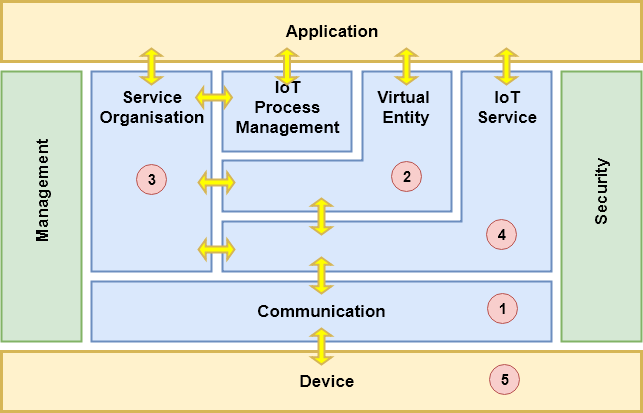
\includegraphics[width=0.8\textwidth]{./Introduction/Chapter1/figures/c1_IoT-A-ARM.png} 
    \caption{Our contributed positions in IoT functional view}
     \label{fig:c1_IoT-A-ARM}
  \end{center} 
\end{figure}


The common IoT architecture provided by Internet of Things Architecture (IoT-A)~\index{IoT-A}\cite{deinternet} and our contributed positions are illustrated in Fig.~\ref{fig:c1_IoT-A-ARM}. For the communication layer, we introduce a method to minimize the effort to establish and configure the connectivity to heterogeneous IoT Things by automatically generating connectors (indexed by number 1 in figure). These connectors also speed up the data acquisition from open data sharing web services. To minimize the error in collecting data from IoT devices, we propose an error and change point detection algorithm powered by active learning as a IoT service (indexed by number 4 in figure). After cleaning data, we try to maximize acquired information from this data by proposing a virtual sensor framework that simplifies creating and configuring VSs with the programmable operators (rule, formula or function) (indexed by number 2 in figure). To increase the interoperability for IoT applications, we provide a descriptive language, which semantically describes not only single Things but also group of Things (indexed by number 3 in figure). To enhance IoT device reliability, we propose an algorithm minimizing energy consumption by real-time estimating the optimal data collection frequency based on historical data (indexed by number 5 in figure). In summary, our contribution spreads on most of the layer of IoT architecture. 


% As consequences of rapid growth, there is a vast amount of raw data being continuously collected from billions of interconnected devices. It is necessary to develop techniques that could maximize usable knowledge from raw data. These techniques could not only transform raw data into high-level information but also identify and eliminate data errors. On the other hands, the Things in IoT are heterogeneous from hardware platforms to communication technologies. In addition, the new device types along with their own data format are emerging every day. This triggers the complex interoperability issues that need to be solved to achieve ``everything could be connected anytime from anywhere by anyone'' \cite{serrano2015internet}\\

 

\section{Thesis Contributions and Outline}
The key contributions in this thesis can be summarized as follows:
\subsection{IoT Interoperability Solutions}
\begin{itemize}

\item \textit{A method to inter-operate IoT device connection using connector}: This solution is a novel industrial IOT framework, which supports automatic establishment and configuration process for heterogeneous connectivity by using connectors. In our framework, the connector is a specific code segment that performs the data acquisition process from a specific type of connectivity using protocols like HTTP, MQTT. An APIs supporting CRUD operations (create, read, update, delete) for the connector is also provided. Furthermore, automating connectivity mechanism assists end-user quickly retrieving data from various data sources via particular connectors.

\item \textit{An IoT Framework to maximize usable knowledge using virtual sensor}: This framework simplifies creating and configuring virtual sensors (VSs) with the programmable operators such as rule, formula or function. These VSs are linked together to be a logical data-flow (LDF) that enables producing the high-level information from collected data. On the top of the framework, a Virtual Sensor Editor (VSE) is also implemented to facilitate building and configuring the LDF by offering the drag-drop actions on HTML5 web interface. In order to achieve scalability and performance, we implement our propose based on clustering architecture along with various strategies such as executing LDF following asynchronous model, using a No-SQL database to store and query data

\item \textit{A semantically Descriptive Language for Group of Things}: It allows to semantically present compound objects namely Asset in Massive IoT scenario. Our method is based on a novel semantic description named Web of Things – Asset Description and a light-weight Web of Things framework, which are fully integrated together for maximizing the interoperability. Such combination is not only capable of presenting, accessing and managing the Asset but also speed up the development of applications.

\end{itemize}

\begin{figure}[h!] 
 \begin{center} 
 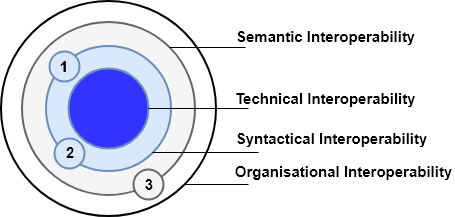
\includegraphics[width=0.7\textwidth]{./Introduction/Chapter1/figures/c1_IoT_contribution_interoperability.png} 
    \caption{Our contributed positions in IoT Interoperability}
     \label{fig:c1_IoT_contribution_interoperability}
  \end{center} 
\end{figure}

\subsection{IoT Reliability Solutions}
\begin{itemize}
\item \textit{An Active Learning method for errors and events detection in time series.}:  This method effectively detects both errors and events in a single algorithm powered by active learning. For the detection, we introduce a non-parametric algorithm, which accurately detects and labels anomalies with a novel concept of neighborhood, and unsupervised probabilistic classification. The detection quality is controlled by the confidence of the classification, which is then used as termination condition for the active learning algorithm. 

\item \textit{An Energy Efficient Sampling Algorithm}: This algorithm minimizes energy consumption by real-time estimating the optimal data collection frequency based on historical data. This frequency is significantly lower than fixed one while maintaining similar data quality. We also demonstrate that our proposal is light-weight enough to be deployed on constraint IoT devices that are limited in computation power and storage.   
\end{itemize}


The work presented in this thesis is structured as follows. Apart from the introduction and final conclusion, we divide the main content into three parts. We present the background knowledge and related works in the first part. Then, in part \ref{pa:part2} and \ref{pa:part3}, we discuss the solution for the interoperability and reliability issues in IoT.

\begin{enumerate}
\item In the first part, we provide the fundamental knowledge of IoT, especially CloudIoT paradigm. This part also highlights the current issues and challenges relating to interoperability and reliability in IoT. Then, the main approaches to deal with these challenges are analyzed in detail to show their advantages and limitation. Base on this analysis, we introduce our solution for the existing issues in the next parts. 

\item The second part discusses several issues regarding Interoperability in IoT. Chapter \ref{ch:connector} presents a solution to facilitate the connectivity to heterogeneous IoT Things. Chapter \ref{ch:Wot-AD} discusses the interoperability for IoT Things and propose a  descriptive language to semantically describes not only single Things but also group of Things.

Results have been presented and/or published
\begin{enumerate}
\item at 3rd IEEE International Forum on Research and Technologies for Society and Industry 2017 (RTSI)~\cite{kim2017industrial}
\item  at 2017 IEEE 13th International Conference on Wireless and Mobile Computing, Networking and Communications (WiMob)~\cite{kim2017scalable}
\end{enumerate}

\item In the last part, we focus on the solutions to increase the reliability in IoT. In chapter \ref{ch:CABD}, we present an errors and change point detection algorithm using active learning. Then, in chapter \ref{ch:smart_freq}, we propose an adaptive sampling algorithm to minimizing the energy consumption in IoT devices.

Results have been presented and / or published
\begin{enumerate}
\item at patent 1
\item at patent 2
\end{enumerate}

\end{enumerate}
